\documentclass[10pt]{article}
\usepackage[margin=1.4cm]{geometry}
\usepackage[default]{sourcesanspro}
\usepackage{xcolor}
\usepackage{tikz}
\usetikzlibrary{arrows.meta, positioning, trees, shapes.geometric}
\usepackage{pgfplots}
\pgfplotsset{compat=1.18}
\pagestyle{empty}
\setlength{\parindent}{0pt}

\definecolor{accent}{HTML}{5B3A8A}
\definecolor{panel}{HTML}{FAF8FC}
\color{black!85}

\newcommand{\panel}[2]{%
  \begin{minipage}[t][5.1cm][t]{0.31\textwidth}
    \centering
    {\bfseries\color{accent} #1}\\[0.3em]
    #2
  \end{minipage}}

\begin{document}

{\LARGE\bfseries\color{accent} TikZ Gallery}\\[0.1em]
{\large Six small figures drawn entirely in TikZ and pgfplots.}

\vspace{1.2em}
\noindent
\panel{Graph}{%
  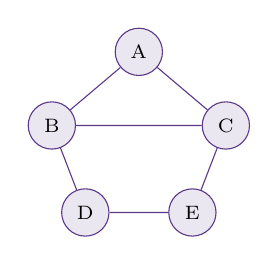
\begin{tikzpicture}[scale=0.85, every node/.style={circle, draw=accent, fill=accent!12,
      minimum size=6mm, font=\scriptsize}]
    \node (a) at (0,1.4) {A};
    \node (b) at (-1.3,0.3) {B};
    \node (c) at (1.3,0.3) {C};
    \node (d) at (-0.8,-1.0) {D};
    \node (e) at (0.8,-1.0) {E};
    \draw[accent] (a)--(b) (a)--(c) (b)--(d) (b)--(c) (c)--(e) (d)--(e);
  \end{tikzpicture}}
\hfill
\panel{Tree}{%
  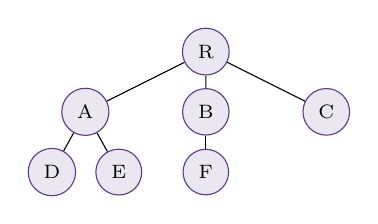
\begin{tikzpicture}[scale=0.85,
      level distance=9mm,
      level 1/.style={sibling distance=18mm},
      level 2/.style={sibling distance=10mm},
      every node/.style={circle, draw=accent, fill=accent!12, minimum size=5mm, font=\scriptsize}]
    \node {R}
      child { node {A}
        child { node {D} }
        child { node {E} } }
      child { node {B}
        child { node {F} } }
      child { node {C} };
  \end{tikzpicture}}
\hfill
\panel{Circuit}{%
  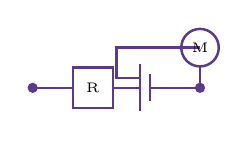
\begin{tikzpicture}[scale=0.85, line width=0.9pt, accent]
    \draw (-1.6,0) -- (-1.0,0);
    \draw (-1.0,-0.3) rectangle (-0.4,0.3);
    \node[font=\tiny, black] at (-0.7,0) {R};
    \draw (-0.4,0) -- (0.0,0);
    \draw (0.0,-0.35) -- (0.0,0.35);
    \draw (0.15,-0.2) -- (0.15,0.2);
    \draw (0.0,0.15) -- (-0.35,0.15) -- (-0.35,0.6) -- (0.9,0.6);
    \draw (0.15,0) -- (0.9,0);
    \draw (0.9,0.6) circle (0.28);
    \node[font=\tiny, black] at (0.9,0.6) {M};
    \draw (0.9,0) -- (0.9,0.32);
    \foreach \x in {-1.6,-1.5,...,-1.0} { }
    \draw[fill=accent] (-1.6,0) circle (1.6pt);
    \draw[fill=accent] (0.9,0) circle (1.6pt);
  \end{tikzpicture}}

\vspace{0.8em}
\noindent
\panel{Plot}{%
  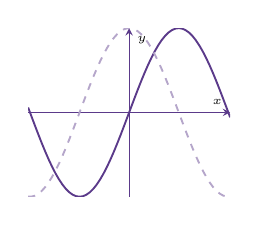
\begin{tikzpicture}[scale=0.85]
    \begin{axis}[width=4.6cm, height=4.1cm, axis lines=middle,
        xlabel={\tiny $x$}, ylabel={\tiny $y$}, ticklabel style={font=\tiny},
        xtick=\empty, ytick=\empty, samples=60, domain=-3.2:3.2,
        axis line style={accent}, tick style={accent}]
      \addplot[accent, thick] {sin(deg(x))};
      \addplot[accent!45, thick, dashed] {cos(deg(x))};
    \end{axis}
  \end{tikzpicture}}
\hfill
\panel{Flowchart}{%
  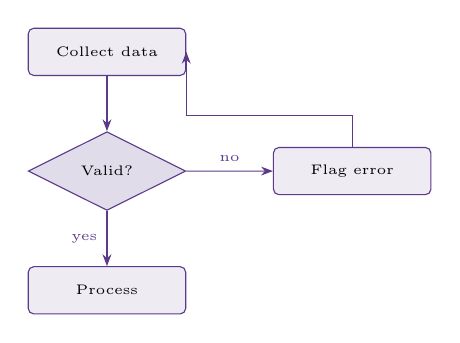
\begin{tikzpicture}[scale=0.8, node distance=7mm,
      every node/.style={font=\tiny},
      box/.style={draw=accent, fill=accent!10, rounded corners=2pt, minimum width=2.0cm, minimum height=6mm, align=center},
      diamond/.style={draw=accent, fill=accent!18, shape=diamond, minimum width=2.0cm, minimum height=1.0cm, align=center, inner sep=0pt},
      arr/.style={-{Stealth[length=1.5mm]}, accent}]
    \node[box] (start) {Collect data};
    \node[diamond, below=of start] (chk) {Valid?};
    \node[box, below=of chk] (proc) {Process};
    \node[box, right=1.1cm of chk] (fix) {Flag error};
    \draw[arr] (start) -- (chk);
    \draw[arr] (chk) -- (proc) node[midway, left, font=\tiny] {yes};
    \draw[arr] (chk) -- (fix) node[midway, above, font=\tiny] {no};
    \draw[arr] (fix.north) -- ++(0,0.5) -| (start.east);
  \end{tikzpicture}}
\hfill
\panel{Mandala}{%
  
\begin{tikzpicture}[scale=0.85]
    \foreach \r in {0.3, 0.6, ..., 1.5} {
      \draw[accent!60] (0,0) circle (\r);
    }
    \foreach \a in {0, 30, ..., 330} {
      \draw[accent, line width=0.5pt] (0,0) -- (\a:1.5);
      \filldraw[accent] (\a:1.5) circle (1.1pt);
      \draw[accent!70] (\a:0.75) circle (0.22);
    }
  \end{tikzpicture}}

\end{document}
